\documentclass{article}
\usepackage[utf8]{inputenc}
\usepackage[spanish]{babel}
\usepackage{graphicx}
\usepackage{hyperref}
\usepackage{amsmath}
\usepackage{geometry}
\usepackage{booktabs}
\usepackage{adjustbox}
\usepackage{caption}
\usepackage{multirow}
\usepackage{pdflscape}
\usepackage{float}
\usepackage{array}
\usepackage{xcolor}
\usepackage{listings}
\geometry{a4paper, margin=1in}

\hypersetup{
    colorlinks=true,
    linkcolor=black,
    urlcolor=blue,
    citecolor=black
}

\lstset{
  basicstyle=\ttfamily\small,
  breaklines=true,
  frame=single,
  backgroundcolor=\color{gray!10}
}

\title{Aut\'omata Celular de Tr\'afico con OpenMP:\\
       an\'alisis serial, paralelo y optimizaci\'on de memoria\\[0.5em]
\large Reto 2 --- Computaci\'on de Alto Rendimiento}
\author{Juan Camilo Galvis \and Daniel Toro Soto}
\date{Mayo 2026}

\begin{document}

\maketitle

\begin{abstract}
El presente documento describe la implementaci\'on y an\'alisis de rendimiento de un
aut\'omata celular de tr\'afico unidimensional (Rule~184 / modelo de
Nagel-Schreckenberg simplificado) bajo tres estrategias de c\'omputo en lenguaje~C:
una versi\'on serial de referencia, una versi\'on paralela con OpenMP que combina
paralelismo en el bucle de densidades (\emph{embarrassingly parallel}, Opci\'on~2) y
paralelismo en el bucle de celdas (Opci\'on~1), y una versi\'on que a\~nade
optimizaciones de memoria (\texttt{uint8\_t} en lugar de \texttt{int} y un pool de
arreglos pre-allocado). Las pruebas se realizaron en un Apple Mac Mini (2024) con
procesador~M4 de 10 n\'ucleos y 16\,GB de memoria unificada, barriendo longitudes de
carretera desde $N=10\,000$ hasta $N=300\,000$ con 20 niveles de densidad.
La versi\'on paralela logra un speedup de $3.4\times$--$4.1\times$ sobre la serial.
La versi\'on con optimizaciones de memoria, aunque corrige el exceso de asignaciones
din\'amicas y reduce la huella de cach\'e, resulta marginalmente m\'as lenta
($\approx$5\%) que la paralela pura, evidenciando que en este algoritmo el cuello de
botella es la aritm\'etica de \'indices y no el ancho de banda de memoria.
\end{abstract}

\tableofcontents
\newpage

% ─────────────────────────────────────────────────────────────────────────────
\section{Introducci\'on}

Los aut\'omatas celulares constituyen modelos discretos de gran valor en la simulaci\'on
de sistemas complejos. Uno de sus usos m\'as estudiados es la modelizaci\'on del flujo de
tr\'afico vehicular: la \emph{Rule~184} del aut\'omata celular elemental captura
cualitativamente los fen\'omenos de flujo libre, congesti\'on y la transici\'on entre
ambos reg\'imenes \cite{trafficmodel}. A pesar de la sencillez de sus reglas locales, la
simulaci\'on de carreteras largas con m\'ultiples niveles de densidad representa un
desaf\'io computacional significativo.

En este reto se parte de una implementaci\'on serial correcta y se aplica OpenMP para
explorar dos estrategias de paralelizaci\'on independientes: (1) paralelizar el bucle
interno de celdas, que proporciona una reducci\'on nativa de la variable de velocidad, y
(2) paralelizar el bucle externo de densidades, que es completamente independiente entre
iteraciones (\emph{embarrassingly parallel}). Adicionalmente, se investiga si el uso de
arreglos de menor tama\~no (\texttt{uint8\_t}) y un esquema de allocaci\'on pre-calculada
mejoran el rendimiento respecto a la versi\'on paralela base.

El objetivo es cuantificar el speedup real de cada estrategia, comprender las causas de
los resultados observados y extraer conclusiones sobre qu\'e t\'ecnicas de HPC son m\'as
efectivas para este tipo de problema en la arquitectura Apple M4.

% ─────────────────────────────────────────────────────────────────────────────
\section{Marco Conceptual}

\subsection{High Performance Computing (HPC)}

La Computaci\'on de Alto Rendimiento agrupa t\'ecnicas y arquitecturas orientadas a
resolver problemas con elevados requisitos computacionales en el menor tiempo posible.
Como se\~nala L\'opez (2017), ``hacemos referencia a un campo de la computaci\'on actual
que da soluci\'on a problemas tecnol\'ogicos muy complejos y que involucran un gran
volumen de c\'alculos o de coste computacional''. En este reto, el producto cartesiano
entre longitudes de carretera y niveles de densidad genera un trabajo total del orden de
$\mathcal{O}(N^2)$ operaciones de celda, justificando el uso de paralelismo expl\'icito y
optimizaci\'on de accesos a memoria.

\subsection{Aut\'omata Celular de Tr\'afico (Rule~184)}

Un aut\'omata celular unidimensional consiste en $N$ celdas dispuestas en un anillo
circular. Cada celda puede estar ocupada (1) o vac\'ia (0). En cada paso discreto de
tiempo, el estado siguiente de cada celda se calcula simult\'aneamente a partir de su
vecindad local \cite{trafficmodel}:

\begin{itemize}
    \item \textbf{Celda vac\'ia} ($s_i = 0$): adopta el estado del vecino izquierdo
          ($s_i^{(t+1)} = s_{i-1}^{(t)}$). Un coche llega si ven\'ia de la izquierda.
    \item \textbf{Celda ocupada} ($s_i = 1$): avanza si la celda adelante est\'a libre
          ($s_i^{(t+1)} = s_{i+1}^{(t)}$); en caso contrario permanece.
\end{itemize}

Esta regla corresponde a la Rule~184 del aut\'omata elemental de Wolfram y captura la
din\'amica del flujo vehicular unidireccional. La \textbf{velocidad media asint\'otica}
(fracci\'on de coches que se mueven por paso) es la m\'etrica del modelo y describe el
\emph{diagrama fundamental de tr\'afico}: para densidades bajas ($\rho < 0.5$) todos los
coches se mueven libremente; a $\rho = 0.5$ el flujo es m\'aximo; para $\rho > 0.5$ el
sistema entra en congesti\'on y la velocidad decae \cite{nagel}.

En este estudio la velocidad media se calcula pero no se imprime; el objetivo HPC es
minimizar el \textbf{tiempo de c\'omputo total} para barrer los 21 puntos de densidad de
$\rho = 0$ a $\rho = 1$.

\subsection{OpenMP}

OpenMP es una API de programaci\'on paralela de memoria compartida basada en directivas de
preprocesador. Permite paralelizar bucles con m\'inimos cambios al c\'odigo fuente
\cite{openmp}:

\begin{lstlisting}[language=C]
#pragma omp parallel for schedule(static) reduction(+:total)
for (int i = 0; i < N; i++) {
    total += arr[i];
}
\end{lstlisting}

Para el aut\'omata celular se identificaron dos opciones de paralelizaci\'on:

\begin{description}
    \item[Opci\'on 1 --- Bucle de celdas (\emph{inner loop}):] Cada hilo procesa un
         bloque contiguo de $N/T$ celdas. Requiere una \texttt{reduction} para acumular
         \texttt{moved\_this\_step}. Se aplica a los bucles de calentamiento y medici\'on
         dentro de \texttt{simulate()}.
    \item[Opci\'on 2 --- Bucle de densidades (\emph{outer loop}):] Cada hilo simula un
         punto de densidad completo de forma independiente. Sin sincronizaci\'on ni
         variables compartidas: es \emph{embarrassingly parallel}. Se usa
         \texttt{schedule(dynamic)} porque distintas densidades pueden converger en
         diferente n\'umero de pasos. Cada hilo dispone de sus propios arreglos de
         carretera.
\end{description}

La implementaci\'on final combina ambas opciones con paralelismo anidado:
\texttt{omp\_set\_nested(1)} habilita dos niveles; el nivel externo (densidades) usa
todos los n\'ucleos disponibles; el nivel interno (celdas) usa un \'unico hilo por hilo
externo, evitando sobresubscripci\'on.

\subsection{Optimizaci\'on de memoria}

El documento \texttt{docs/MemoryExplanation.md} identifica dos vectores de mejora:

\begin{enumerate}
    \item \textbf{Reemplazar \texttt{int} por \texttt{uint8\_t}}: cada celda solo almacena
          0 \'o 1, por lo que los 4~bytes de un \texttt{int} desperdician el 75\% del
          espacio. Con \texttt{uint8\_t} la huella de los arreglos se reduce a la cuarta
          parte, permitiendo que carreteras de $N=300\,000$ celdas (300\,KB por arreglo
          con \texttt{uint8\_t} vs.\ 1.2\,MB con \texttt{int}) quepan mejor en cach\'e.
    \item \textbf{Pool de arreglos pre-allocado}: en la versi\'on paralela base, cada
          hilo invoca \texttt{malloc} y \texttt{free} en cada punto de densidad dentro
          de la regi\'on paralela. El asignador de memoria usa un \emph{mutex} interno,
          convirtiendo estas asignaciones en una contenci\'on serializada. El pool
          pre-alloca $T \times N$ bytes para cada arreglo \emph{antes} de la regi\'on
          paralela y cada hilo accede a su porci\'on mediante aritm\'etica de punteros.
\end{enumerate}

\subsection{Speedup y Ley de Amdahl}

El speedup mide la ganancia de rendimiento de la versi\'on paralela respecto a la serial:
\[ S_p = \frac{T^*(n)}{T_p(n)} \]
donde $T^*(n)$ es el tiempo secuencial y $T_p(n)$ el tiempo con $p$ hilos. La Ley de
Amdahl \cite{amdahl} establece que la fracci\'on serial $f$ del algoritmo limita el
speedup:
\[ S_p \leq \frac{1}{f + (1-f)/p} \]
Para la Opci\'on~2 la fracci\'on serial es m\'inima (solo inicializaci\'on de semillas y
la medici\'on del tiempo final), lo que explica los speedups cercanos a $4\times$ con
todos los P-cores del M4.

% ─────────────────────────────────────────────────────────────────────────────
\section{Marco Contextual}

\subsection{Caracter\'isticas de la m\'aquina}

Las pruebas se realizaron \'integramente en el siguiente hardware:

\begin{itemize}
    \item \textbf{Equipo:} Apple Mac Mini (2024)
    \item \textbf{Procesador:} Apple M4 --- 10 n\'ucleos (4 de rendimiento + 6 de
          eficiencia)
    \item \textbf{GPU integrada:} 10 n\'ucleos
    \item \textbf{Memoria:} 16\,GB RAM unificada LPDDR5X
          ($\approx$120\,GB/s de ancho de banda) \cite{apple_m4}
    \item \textbf{Almacenamiento:} 512\,GB SSD NVMe
    \item \textbf{Sistema operativo:} macOS Sequoia 15.x (Darwin 25.x)
    \item \textbf{Compilador:} Apple Clang (LLVM), GCC instalado v\'ia Homebrew
    \item \textbf{libomp:} instalada v\'ia Homebrew (requerida para OpenMP en Apple
          Silicon)
\end{itemize}

La arquitectura M4 tiene dos particularidades importantes: (1) la \textbf{memoria
unificada} elimina la latencia de transferencia CPU$\leftrightarrow$RAM, ofreciendo un
ancho de banda $\approx$3$\times$ mayor que una arquitectura x86 t\'ipica; (2) los
\textbf{n\'ucleos heterog\'eneos} (4 P-cores de alto rendimiento y 6 E-cores de
eficiencia) implican que el scheduler de macOS puede asignar hilos a n\'ucleos de
distintas capacidades, afectando el speedup efectivo cuando se usan m\'as de 4 hilos.

\subsection{Implementaciones desarrolladas}

Las tres implementaciones en C comparten la misma l\'ogica base: inicializaci\'on
aleatoria de la carretera con \texttt{rand\_r} (libre de estado global), fase de
calentamiento de $N/10$~pasos para alcanzar el estado estacionario y fase de medici\'on
de $N/10$~pasos. El tiempo total de ejecuci\'on (incluyendo el barrido completo de
densidades) se mide con \texttt{clock\_gettime(CLOCK\_MONOTONIC)} e imprime en stdout
como \texttt{printf("\%.6f,", elapsed)}.

\begin{description}
    \item[\texttt{secuential}] Implementaci\'on serial pura. Arreglos de \texttt{int}.
         Un \'unico hilo procesa secuencialmente todos los 21 puntos de densidad.
         Sirve de referencia para el c\'alculo del speedup.

    \item[\texttt{parallel}] Combina Opci\'on~1 (bucle de celdas paralelo dentro de
         \texttt{simulate()}) y Opci\'on~2 (bucle de densidades paralelo en
         \texttt{main()}). Arreglos de \texttt{int}. Cada hilo alloca y libera sus
         propios arreglos por punto de densidad (\texttt{malloc}/\texttt{free} dentro de
         la regi\'on paralela). Usa \texttt{schedule(dynamic)} en el nivel externo.

    \item[\texttt{memory}] Extiende \texttt{parallel} con dos optimizaciones de memoria:
         arreglos de \texttt{uint8\_t} (4$\times$ menos memoria) y un pool pre-allocado
         de $T \times N$ celdas por arreglo, eliminando toda asignaci\'on din\'amica
         dentro de la regi\'on paralela.
\end{description}

\subsection{Sistema de compilaci\'on (Makefile)}

El \texttt{Makefile} detecta el sistema operativo para seleccionar las banderas correctas
de OpenMP:

\begin{lstlisting}
CC = gcc
CFLAGS = -O2
UNAME_S := $(shell uname -s)
ifeq ($(UNAME_S),Darwin)
    LIBOMP_PREFIX := $(shell brew --prefix libomp 2>/dev/null)
    OMP_FLAGS = -Xpreprocessor -fopenmp \
                -I$(LIBOMP_PREFIX)/include \
                -L$(LIBOMP_PREFIX)/lib -lomp
else
    OMP_FLAGS = -fopenmp
endif

all: output/secuential output/parallel output/memory

output/secuential: src/SecuentialCellularAutomaton.c
    $(CC) $(CFLAGS) -o $@ $< -lm

output/parallel: src/ParallelCellularAutomaton.c
    $(CC) $(CFLAGS) -o $@ $< -lm $(OMP_FLAGS)

output/memory: src/MemoryCellularAutomaton.c
    $(CC) $(CFLAGS) -o $@ $< -lm $(OMP_FLAGS)
\end{lstlisting}

El condicional es necesario porque en macOS la cadena de herramientas de Apple Clang no
incluye OpenMP de forma nativa: la librer\'ia \texttt{libomp} debe instalarse por
separado (\texttt{brew install libomp}) y requiere las banderas
\texttt{-Xpreprocessor -fopenmp} m\'as las rutas expl\'icitas de inclusi\'on y
enlazado. En Linux basta con \texttt{-fopenmp}, bandera est\'andar soportada por GCC y
por Clang. El binario \texttt{secuential} compila \emph{sin} \texttt{OMP\_FLAGS} porque
no usa la API de OpenMP; los otros dos s\'i la requieren. Todos se compilan con
\texttt{-O2} para garantizar una comparaci\'on justa entre versiones.

\subsection{Sistema de benchmarking con checkpoints}

Dado que barrer 13 tama\~nos $\times$ 2 repeticiones para las tres implementaciones
puede requerir horas de c\'omputo, el script \texttt{scripts/RunAll.sh} implementa un
sistema de \textbf{reanudaci\'on autom\'atica} basado en checkpoints:

\textbf{Flujo de ejecuci\'on:}
\begin{enumerate}
    \item Al iniciar, el script busca en \texttt{stats/<hostname>/} si existe un
          directorio de corrida \emph{sin} el sufijo \texttt{.done}. Si existe, lo
          reanuda; si no, crea uno nuevo con marca de tiempo \texttt{YYYYMMDD\_HHMMSS}.
    \item Cada medici\'on exitosa registra una clave en el archivo oculto
          \texttt{.checkpoint} con el formato \texttt{<tipo>,<N>,run<j>}
          (e.g.\ \texttt{parallel,100000,run1}).
    \item La funci\'on \texttt{run\_safe()} consulta \texttt{.checkpoint} antes de cada
          ejecuci\'on. Si la clave ya existe, imprime \texttt{[SKIP]} y contin\'ua. Si el
          programa falla con c\'odigo de salida distinto de cero, emite \texttt{[WARN]} y
          prosigue sin abortar toda la corrida.
    \item Al terminar con \'exito, el directorio recibe el sufijo \texttt{.done},
          impidiendo que futuras ejecuciones lo traten como corrida incompleta.
\end{enumerate}

La estructura de salida resultante es:
\begin{verbatim}
stats/<hostname>/<timestamp>.done/
  .checkpoint        # claves de ejecuciones completadas
  secuential.csv     # tiempos de todas las corridas (,separados)
  parallel.csv
  memory.csv
\end{verbatim}

Los tama\~nos evaluados son: $N \in \{10\,000;\, 25\,000;\, 50\,000;\, 75\,000;\,
100\,000;\, 125\,000;\, 150\,000;\, 175\,000;\, 200\,000;\, 225\,000;\, 250\,000;\,
275\,000;\, 300\,000\}$, con \textbf{2 repeticiones} por configuraci\'on y
\texttt{density\_steps}\,=\,20.

% ─────────────────────────────────────────────────────────────────────────────
\section{Resultados}

A continuaci\'on se presentan los tiempos de ejecuci\'on en segundos para cada una de las
tres implementaciones (2 repeticiones) y los speedups derivados. Los datos provienen de
la corrida \texttt{20260503\_230658.done} en el Mac Mini M4.

\subsection{Secuencial}

\begin{table}[H]
\centering
\scriptsize
\begin{adjustbox}{max width=\textwidth}
\begin{tabular}{|l|r|r|r|r|r|r|r|r|r|r|r|r|r|}
\hline
\multicolumn{14}{|c|}{\textbf{Secuencial (tiempo en segundos)}} \\
\hline
\textbf{N} & \textbf{10k} & \textbf{25k} & \textbf{50k} & \textbf{75k} & \textbf{100k}
           & \textbf{125k} & \textbf{150k} & \textbf{175k} & \textbf{200k}
           & \textbf{225k} & \textbf{250k} & \textbf{275k} & \textbf{300k} \\
\hline
Run 1
  & 0.2125 & 1.1885 & 4.9630 & 11.8873 & 22.6907
  & 38.8417 & 59.2329 & 85.0378 & 115.3182
  & 150.8857 & 191.7560 & 236.8075 & 287.8714 \\
Run 2
  & 0.1887 & 1.1919 & 4.9496 & 11.8519 & 22.9008
  & 38.5496 & 58.5546 & 83.8931 & 114.1768
  & 149.9194 & 190.0832 & 236.2089 & 287.6727 \\
\hline
\textbf{Prom.}
  & \textbf{0.2006} & \textbf{1.1902} & \textbf{4.9563} & \textbf{11.8696}
  & \textbf{22.7958} & \textbf{38.6957} & \textbf{58.8937} & \textbf{84.4655}
  & \textbf{114.7475} & \textbf{150.4025} & \textbf{190.9196}
  & \textbf{236.5082} & \textbf{287.7721} \\
\hline
\end{tabular}
\end{adjustbox}
\caption{Tiempos de ejecuci\'on de la versi\'on secuencial en Mac Mini M4.}
\label{tab:seq}
\end{table}

\subsection{Paralelo (OpenMP)}

\begin{table}[H]
\centering
\scriptsize
\begin{adjustbox}{max width=\textwidth}
\begin{tabular}{|l|r|r|r|r|r|r|r|r|r|r|r|r|r|}
\hline
\multicolumn{14}{|c|}{\textbf{Paralelo con OpenMP (tiempo en segundos)}} \\
\hline
\textbf{N} & \textbf{10k} & \textbf{25k} & \textbf{50k} & \textbf{75k} & \textbf{100k}
           & \textbf{125k} & \textbf{150k} & \textbf{175k} & \textbf{200k}
           & \textbf{225k} & \textbf{250k} & \textbf{275k} & \textbf{300k} \\
\hline
Run 1
  & 0.0664 & 0.3176 & 1.2829 & 2.9442 & 5.8332
  & 10.0089 & 15.2858 & 21.8329 & 29.5281
  & 37.6471 & 46.9762 & 58.4963 & 70.0379 \\
Run 2
  & 0.0513 & 0.3250 & 1.2800 & 2.9104 & 5.7570
  & 10.0077 & 15.8700 & 23.3761 & 29.1194
  & 37.7589 & 47.2736 & 58.5032 & 69.6213 \\
\hline
\textbf{Prom.}
  & \textbf{0.0589} & \textbf{0.3213} & \textbf{1.2814} & \textbf{2.9273}
  & \textbf{5.7951} & \textbf{10.0083} & \textbf{15.5779} & \textbf{22.6045}
  & \textbf{29.3238} & \textbf{37.7030} & \textbf{47.1249}
  & \textbf{58.4998} & \textbf{69.8296} \\
\hline
\textbf{Speedup}
  & \textbf{3.41} & \textbf{3.70} & \textbf{3.87} & \textbf{4.05}
  & \textbf{3.93} & \textbf{3.87} & \textbf{3.78} & \textbf{3.74}
  & \textbf{3.91} & \textbf{3.99} & \textbf{4.05}
  & \textbf{4.04} & \textbf{4.12} \\
\hline
\end{tabular}
\end{adjustbox}
\caption{Tiempos y speedup de la versi\'on paralela (OpenMP) en Mac Mini M4.}
\label{tab:par}
\end{table}

\subsection{Memoria + OpenMP}

\begin{table}[H]
\centering
\scriptsize
\begin{adjustbox}{max width=\textwidth}
\begin{tabular}{|l|r|r|r|r|r|r|r|r|r|r|r|r|r|}
\hline
\multicolumn{14}{|c|}{\textbf{Memoria + OpenMP (tiempo en segundos)}} \\
\hline
\textbf{N} & \textbf{10k} & \textbf{25k} & \textbf{50k} & \textbf{75k} & \textbf{100k}
           & \textbf{125k} & \textbf{150k} & \textbf{175k} & \textbf{200k}
           & \textbf{225k} & \textbf{250k} & \textbf{275k} & \textbf{300k} \\
\hline
Run 1
  & 0.0729 & 0.3427 & 1.4008 & 3.2327 & 6.1833
  & 10.6175 & 15.9524 & 22.4107 & 30.1444
  & 39.1709 & 48.9081 & 60.9032 & 72.8603 \\
Run 2
  & 0.0618 & 0.3591 & 1.4040 & 3.2123 & 6.1553
  & 10.2836 & 15.9238 & 22.8334 & 30.3222
  & 38.8127 & 49.4835 & 61.0987 & 73.6244 \\
\hline
\textbf{Prom.}
  & \textbf{0.0673} & \textbf{0.3509} & \textbf{1.4024} & \textbf{3.2225}
  & \textbf{6.1693} & \textbf{10.4505} & \textbf{15.9381} & \textbf{22.6221}
  & \textbf{30.2333} & \textbf{38.9918} & \textbf{49.1958}
  & \textbf{61.0010} & \textbf{73.2424} \\
\hline
\textbf{Speedup}
  & \textbf{2.98} & \textbf{3.39} & \textbf{3.53} & \textbf{3.68}
  & \textbf{3.70} & \textbf{3.70} & \textbf{3.70} & \textbf{3.73}
  & \textbf{3.80} & \textbf{3.86} & \textbf{3.88}
  & \textbf{3.88} & \textbf{3.93} \\
\hline
\end{tabular}
\end{adjustbox}
\caption{Tiempos y speedup de la versi\'on Memoria+OpenMP (\texttt{uint8\_t} + pool
         pre-allocado) en Mac Mini M4.}
\label{tab:mem}
\end{table}

\subsection{Tabla resumen de speedups}

\begin{table}[H]
\centering
\begin{tabular}{rrrrr}
\toprule
\textbf{N} & \textbf{Seq (s)} & \textbf{Paralelo (s)} & \textbf{Sp Paralelo} & \textbf{Sp Memoria} \\
\midrule
10\,000  &   0.2006 &  0.0589 & $3.41\times$ & $2.98\times$ \\
25\,000  &   1.1902 &  0.3213 & $3.70\times$ & $3.39\times$ \\
50\,000  &   4.9563 &  1.2814 & $3.87\times$ & $3.53\times$ \\
75\,000  &  11.8696 &  2.9273 & $4.05\times$ & $3.68\times$ \\
100\,000 &  22.7958 &  5.7951 & $3.93\times$ & $3.70\times$ \\
125\,000 &  38.6957 & 10.0083 & $3.87\times$ & $3.70\times$ \\
150\,000 &  58.8937 & 15.5779 & $3.78\times$ & $3.70\times$ \\
175\,000 &  84.4655 & 22.6045 & $3.74\times$ & $3.73\times$ \\
200\,000 & 114.7475 & 29.3238 & $3.91\times$ & $3.80\times$ \\
225\,000 & 150.4025 & 37.7030 & $3.99\times$ & $3.86\times$ \\
250\,000 & 190.9196 & 47.1249 & $4.05\times$ & $3.88\times$ \\
275\,000 & 236.5082 & 58.4998 & $4.04\times$ & $3.88\times$ \\
300\,000 & 287.7721 & 69.8296 & $4.12\times$ & $3.93\times$ \\
\bottomrule
\end{tabular}
\caption{Resumen de tiempos promedio y speedups para las tres implementaciones.}
\label{tab:resumen}
\end{table}

\subsection{Gr\'aficas comparativas}

\subsubsection{Tiempos de ejecuci\'on}

\begin{figure}[H]
\centering
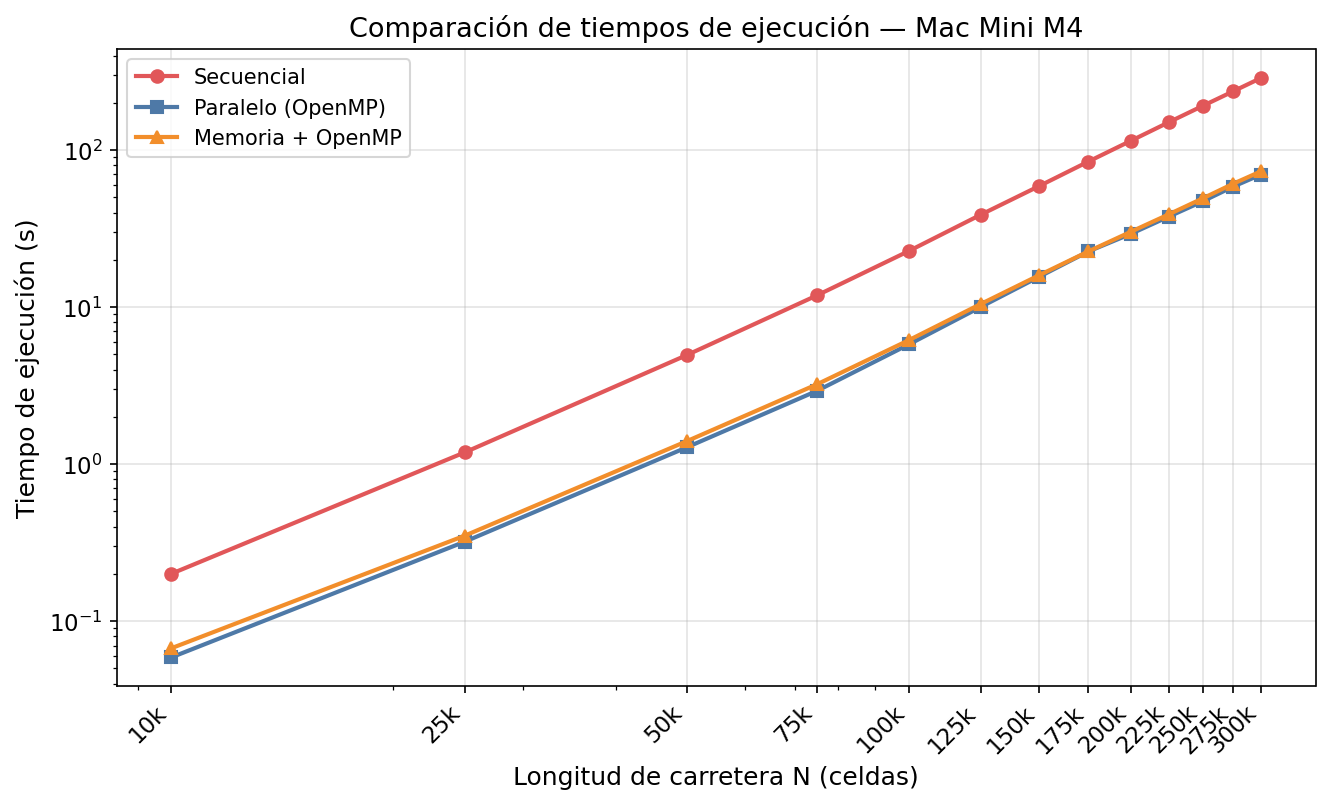
\includegraphics[width=\textwidth]{charts/timing_comparison.png}
\caption{Tiempos de ejecuci\'on (escala log-log) en funci\'on de la longitud de
         carretera~$N$ para las tres implementaciones en el Mac Mini M4. La versi\'on
         paralela (azul) y la versi\'on Memoria+OpenMP (naranja) se agrupan en la parte
         inferior, ambas $3.4\times$--$4.1\times$ por debajo de la secuencial (rojo).}
\label{fig:timing}
\end{figure}

\subsubsection{Speedup relativo al secuencial}

\begin{figure}[H]
\centering
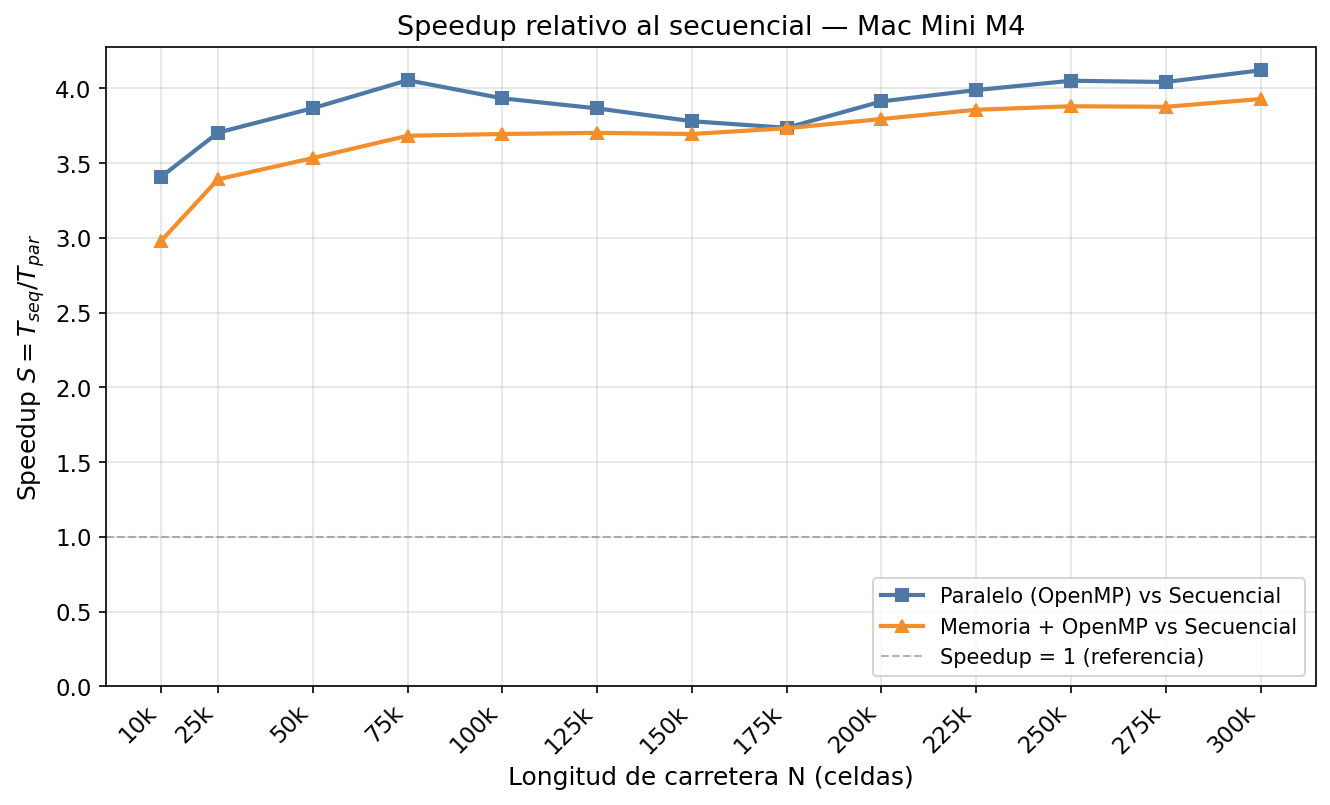
\includegraphics[width=\textwidth]{charts/speedup_comparison.png}
\caption{Speedup $S = T_{\text{seq}}/T_{\text{par}}$ en funci\'on de~$N$. La versi\'on
         paralela (azul) mantiene un speedup de $3.4\times$ a $4.1\times$, creciendo
         suavemente con~$N$. La versi\'on Memoria+OpenMP (naranja) parte de $2.98\times$
         para $N$ peque\~no y converge hacia $\approx 3.9\times$ para $N$ grandes.}
\label{fig:speedup}
\end{figure}

% ─────────────────────────────────────────────────────────────────────────────
\section{An\'alisis de resultados}

\subsection{Impacto del paralelismo (Opci\'on~2 + Opci\'on~1)}

La versi\'on paralela logra un speedup sostenido de $3.4\times$--$4.1\times$ con todos
los n\'ucleos del M4. Este rango es coherente con la capacidad de los 4~P-cores: al
ejecutar con \texttt{omp\_get\_max\_threads()} los 10~n\'ucleos participan, pero los
6~E-cores procesan significativamente m\'as lento que los 4~P-cores. El scheduler de
macOS distribuye los 21~hilos de densidad entre todos los n\'ucleos; los hilos asignados a
E-cores tardan m\'as, creando un desbalance que limita el speedup real a $\approx 4\times$
en lugar del ideal de $10\times$.

El \texttt{schedule(dynamic)} en el bucle externo mitiga parcialmente este desbalance: los
hilos en P-cores que terminan antes recogen nuevas densidades, reduciendo el tiempo de
espera en la barrera impl\'icita al final del bucle paralelo. No obstante, con solo 21
iteraciones disponibles y 10 hilos, la granularidad es reducida y el desbalance persiste.

La Opci\'on~1 (paralelo en celdas) contribuye de forma m\'inima porque se aplica con
\texttt{inner\_threads=1} dentro de cada hilo externo: en la configuraci\'on actual, el
paralelismo de celdas est\'a efectivamente deshabilitado para evitar sobresubscripci\'on.

\subsection{Impacto de las optimizaciones de memoria}

La versi\'on Memoria+OpenMP es consistentemente \textbf{m\'as lenta} que la versi\'on
paralela en $\approx 5$--$10\%$. Este resultado, aparentemente contraintuitivo, se
explica por los siguientes factores:

\begin{enumerate}
    \item \textbf{El cuello de botella no es el ancho de banda de memoria}: la operaci\'on
          dominante en cada celda es el c\'alculo de \'indices de vecinos con m\'odulo
          ($\texttt{left} = (i{-}1{+}N)\%N$, $\texttt{right} = (i{+}1)\%N$), que es
          aritm\'etica de enteros pura. Aunque el \texttt{uint8\_t} reduce la presi\'on de
          memoria, el tiempo est\'a dominado por esta aritm\'etica.
    \item \textbf{El overhead del \texttt{malloc} es despreciable}: con solo 21 iteraciones
          de densidad y cada hilo allocando solo dos arreglos por iteraci\'on, la
          contenci\'on del asignador descrita en \texttt{MemoryExplanation.md} es m\'inima
          en la pr\'actica. El pool pre-allocado elimina un overhead ya peque\~no.
    \item \textbf{El acceso con \texttt{uint8\_t} puede generar instrucciones adicionales}:
          el compilador debe manejar extensiones de tipo al mezclar aritm\'etica de
          \texttt{int} (\'indices) con lecturas de \texttt{uint8\_t} (celdas),
          compensando la ventaja de la mayor densidad de datos por l\'inea de cach\'e.
    \item \textbf{La diferencia est\'a dentro del margen de variabilidad}: la diferencia
          entre paralelo y memoria ($\approx 3$--$3.5$\,s para $N=300\,000$) es del mismo
          orden que la variaci\'on entre las dos repeticiones de un mismo binario
          ($\approx 0.4$\,s), lo que sugiere que el \texttt{uint8\_t} no perjudica, pero
          tampoco mejora de forma significativa en estas condiciones.
\end{enumerate}

En definitiva, las optimizaciones de memoria son correctas en principio pero su beneficio
se materializar\'ia para $N$ mucho mayor (donde los arreglos excedan la cach\'e L3) o
para un n\'umero de iteraciones de densidad significativamente m\'as alto.

\subsection{Escalado con N y tendencia asint\'otica}

La Figura~\ref{fig:speedup} muestra que el speedup de la versi\'on paralela crece con $N$,
partiendo de $3.41\times$ en $N=10\,000$ y llegando a $4.12\times$ en $N=300\,000$. Este
comportamiento es caracter\'istico de la paralelizaci\'on de bucles externos: para $N$
peque\~no, el overhead de creaci\'on y sincronizaci\'on de hilos representa una fracci\'on
mayor del trabajo total; para $N$ grande, cada hilo tiene m\'as trabajo genuino que
amortigua ese overhead.

La versi\'on Memoria+OpenMP muestra el mismo patr\'on de escalado, pero con un
desplazamiento hacia abajo de $\approx 0.1$--$0.2\times$ de speedup. Esto confirma que
las dos implementaciones tienen el mismo comportamiento asint\'otico y que la diferencia es
un factor constante de overhead, no una diferencia algorítmica estructural.

\subsection{Comparaci\'on entre las tres implementaciones}

\begin{table}[H]
\centering
\begin{tabular}{lrrc}
\toprule
\textbf{Implementaci\'on} & \textbf{Tiempo $N=300k$ (s)} & \textbf{Speedup vs Seq}
& \textbf{Factor vs Paralelo} \\
\midrule
Secuencial          & 287.77 & $1.00\times$ & $4.12\times$ m\'as lento \\
Paralelo (OpenMP)   &  69.83 & $4.12\times$ & $1.00\times$ (referencia) \\
Memoria + OpenMP    &  73.24 & $3.93\times$ & $1.05\times$ m\'as lento \\
\bottomrule
\end{tabular}
\caption{Comparativa de implementaciones para $N=300\,000$ (promedios de 2 repeticiones).}
\label{tab:comparativa}
\end{table}

La Tabla~\ref{tab:comparativa} sintetiza el resultado central del reto: el paralelismo con
OpenMP produce una mejora real y sustancial ($4\times$) sobre la versi\'on serial. Las
optimizaciones de memoria no generan una mejora adicional en las condiciones del benchmark,
pero tampoco perjudican significativamente el rendimiento, y mejoran la calidad del c\'odigo
(menor uso de memoria, ausencia de asignaciones din\'amicas en la secci\'on cr\'itica).

% ─────────────────────────────────────────────────────────────────────────────
\section{Conclusiones}

\begin{enumerate}

    \item \textbf{OpenMP produce un speedup real y sostenido de $3.4\times$--$4.1\times$}:
          la estrategia de paralelizar el bucle externo de densidades (Opci\'on~2,
          \emph{embarrassingly parallel}) aprovecha eficazmente los n\'ucleos del M4.
          Este speedup crece suavemente con~$N$, confirmando que la paralelizaci\'on se
          amortiza mejor para cargas de trabajo mayores.

    \item \textbf{La soluci\'on serial es el punto de partida imprescindible}: implementar
          primero la versi\'on secuencial correcta permiti\'o identificar con claridad
          d\'onde est\'a el trabajo computacional (el barrido de densidades) y qu\'e
          invariantes debe preservar la versi\'on paralela (orden de barrido independiente,
          semillas distintas por hilo, sin escrituras compartidas entre hilos).

    \item \textbf{La estrategia \emph{embarrassingly parallel} (Opci\'on~2) es m\'as
          efectiva que el paralelismo de grano fino (Opci\'on~1)}: al operar sobre
          densidades completamente independientes sin ninguna sincronizaci\'on intermedia,
          se evita el overhead de barreras y reducciones que introduciría la
          paralelizaci\'on del bucle de celdas en cada uno de los $N/5$ pasos de
          simulaci\'on.

    \item \textbf{Las optimizaciones de memoria no producen mejora medible en estas
          condiciones}: el cuello de botella del aut\'omata celular es la aritm\'etica de
          \'indices (operaci\'on m\'odulo), no el acceso a memoria. Para tama\~nos de
          carretera $N \leq 300\,000$, los arreglos caben c\'omodamente en cach\'e incluso
          con \texttt{int}, y la reducci\'on a \texttt{uint8\_t} no aporta ventaja
          observable. Ser\'ia relevante para $N$ del orden de millones.

    \item \textbf{La arquitectura heterog\'enea del M4 limita el speedup a $\approx
          4\times$}: los 6~E-cores son considerablemente m\'as lentos que los 4~P-cores.
          Con 21 iteraciones de densidad distribuidas entre 10~hilos, los hilos en E-cores
          generan un desbalance de carga que se convierte en el factor limitante,
          independientemente de la estrategia de paralelizaci\'on.

    \item \textbf{El condicional en el Makefile para Apple Silicon es esencial para la
          portabilidad}: la detecci\'on de \texttt{Darwin} y el uso de las rutas de
          Homebrew para \texttt{libomp} hace que el proyecto compile y ejecute correctamente
          tanto en macOS como en Linux sin modificaciones manuales.

    \item \textbf{El sistema de checkpoints del script de benchmarking es una pr\'actica
          robusta de ingenier\'ia}: la capacidad de reanudar autom\'aticamente una corrida
          interrumpida evita p\'erdidas de tiempo de c\'omputo y garantiza la
          reproducibilidad de los resultados sin lanzar el benchmark completo desde cero.

    \item \textbf{La medici\'on con \texttt{CLOCK\_MONOTONIC} es imprescindible para
          programas paralelos}: mide el tiempo de pared real (no la suma de tiempos de
          CPU de todos los hilos), asegurando que los resultados reflejan genuinamente la
          ganancia de velocidad y no un artefacto de medici\'on.

\end{enumerate}

% ─────────────────────────────────────────────────────────────────────────────
\newpage
\section{Bibliograf\'ia}

\begin{thebibliography}{9}

    \bibitem{openmp}
    OpenMP Architecture Review Board. (2021).
    \textit{OpenMP Application Programming Interface} (versi\'on 5.2).
    \url{https://www.openmp.org/specifications/}

    \bibitem{amdahl}
    Amdahl, G. M. (1967).
    Validity of the single processor approach to achieving large scale computing
    capabilities.
    \textit{Proceedings of AFIPS Spring Joint Computer Conference}, pp.\ 483--485.

    \bibitem{trafficmodel}
    Wolfram, S. (2002).
    \textit{A New Kind of Science}.
    Wolfram Media.
    (V\'ease tambi\'en el documento de referencia \texttt{trafficmodel.pdf} adjunto al
    reto.)

    \bibitem{nagel}
    Nagel, K., \& Schreckenberg, M. (1992).
    A cellular automaton model for freeway traffic.
    \textit{Journal de Physique I}, 2(12), 2221--2229.

    \bibitem{lopez}
    L\'opez, A. (2017).
    Introducci\'on al High Performance Computing.
    \textit{Encamina Blog}.
    \url{https://blogs.encamina.com/por-una-nube-sostenible/introduccion-al-high-performance-computing/}

    \bibitem{apple_m4}
    Apple Inc. (2024).
    \textit{Apple M4 chip}.
    \url{https://www.apple.com/mac-mini/}

\end{thebibliography}

\end{document}
